%!TEX root = ../thesis.tex
%*******************************************************************************
%****************************** Second Chapter *********************************
%*******************************************************************************

\chapter{Deep Learning}

\ifpdf
     \graphicspath{{Figs/Chapter2/}}
\else
    \graphicspath{{Chapter2/Figs/Vector/}{Chapter2/Figs/}}
\fi

There are many tasks which are hard to write algorithms for. For example, writing an algorithm the identifies a type of fruit using a picture of the fruit is a challenging undertaking. You could try to solve this problem by asking a number of yes or no questions which help whittle down the possibilities to a handful of fruit. A sensible question to ask might be - "Is the fruit round?". If the answer was yes, we could immediately discard options like strawberries, pineapples and pears. Another sensible question to ask might be - "Is the fruit orange?". If the answer is yes, again we could immediately discard unlikely candidates. Finally we could ask - "Is the fruit rough?". And if the answer was no, we could be pretty sure the picture we were looking at was an orange. \newline
The problem with this approach is that it is very brittle. You could ask a question that would lead a high likelihood that the image was indeed an orange, however the image may not in fact be an orange. For example apples could also be round, orange and smooth. More questions could try to disambiguate the two types of fruit, but there is enough variation in fruit that our algorithm could be confused. Writing rules in this way also is not scalable. There are a large number of types of fruits, and writing questions to determine each one quickly becomes intractable, let alone questions that help distinguish similar fruit. \newline 
Machine learning (ML) is used to solve such tasks, as well as others such as weather prediction, stock price forecasting and risk modelling ~\citep{hastie2009elements}. ML is the process of using data to build prediction models where these models typically output discrete (classification) or continuous (regression) values. ML uses a number of learning paradigms ~\citep{murphy2012machine}, including supervised learning, unsupervised learning and reinforcement learning, to train models. The models can be divided into three classes, namely shallow, deep and probabilistic ~\citep{hastie2009elements, murphy2012machine}. The models are trained using data to accomplish a task. \newline
\newpage
This chapter presents a discussion on the supervised learning paradigm, an analysis of the convolutional network ~\citep{lecun1998gradient} and recurrent network ~\citep{werbos1988generalization} deep learning models, and a discussion on deep learning training techniques, including dropout ~\citep{srivastava2014dropout} and batch normalisation ~\citep{ioffe2015batch} regularisation. 


%********************************** %First Section  **************************************

\section{Supervised Learning}

ML prediction models take as input a set of features. These features are attributes of a data sample. For example in the fruit prediction task mentioned above, input features would be the attributes of a fruit. They would include characteristics such as shape, colour, texture and size. These inputs are provided to a model that maps to outputs. In the example above, these outputs would be types of fruit, and could represent values such as oranges, apples, strawberries and pineapples, amongst others. The model is then taught (trained) to identify the correct fruit (output) based on the features (input) it receives. This type of training paradigm is called supervised learning \citep{bishop2006pattern, hastie2009elements, murphy2012machine}. \newline

\begin{figure}[H]
  	\caption{Supervised Learning}
   	\centering
    	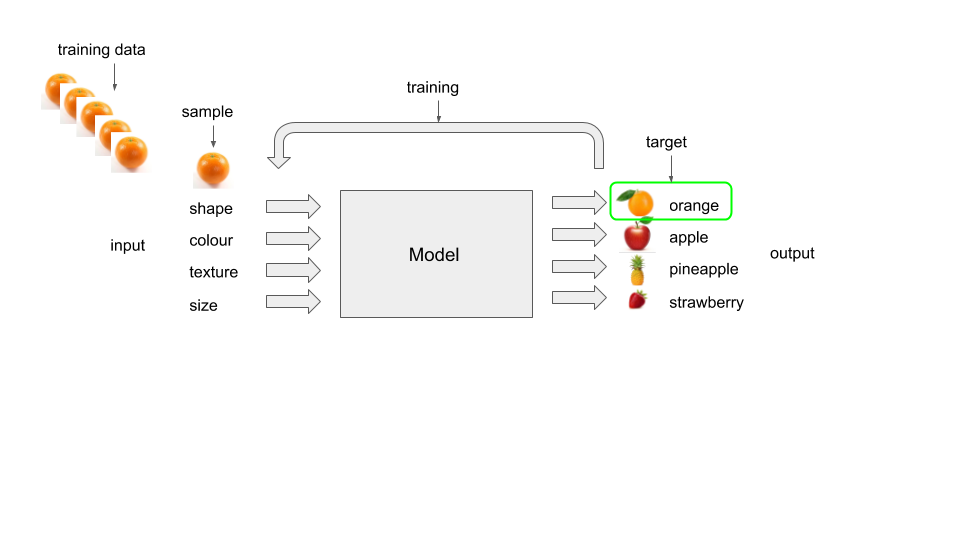
\includegraphics[width=\textwidth]{supervised_learning}
\end{figure}

Features can be continuous valued or discrete, where discrete values are referred to as categorical variables. Outputs can also be continuous or discrete, where discrete outputs are known as classes. Input-output pairs comprise a dataset which is represented as follows, \begin{math} D = \{(x_i, y_i)\}_{i=1}^N \end{math}, where \begin{math} D \end{math} is the dataset, \begin{math} x_i \end{math} is the input sample and \begin{math} y_i \end{math} is the output label. The model has to learn the correct mapping of input to output - features to label. We use data samples to train the model to recognise which features are correlated with which labels. The model is trained using an algorithm where it is shown a sample and it outputs what it believes is the correct label. If it gets the label wrong, an objective function is used to assess how large the error was, and the model is adjusted. We try to minimise this error during training, and because we try to minimise the objective function value, it is called a loss function. The algorithm is expressed as follows: \bigbreak

\begin{algorithm}[H]
	\SetAlgoLined
	\textbf{Input} 
	Training set \begin{math} D = \{(x_i, y_i)\}_{i=1}^N \end{math}, samples and labels\;
  	\begin{math} S_{batch} \gets sample(S, b) \end{math} // sample a minibatch of size \begin{math} b \end{math} \\
	 \For{(x, y) \begin{math} \in S_{batch} \end{math}}{
     		\begin{math} y \gets predict(x, y) \end{math} // predict label for sample \\
		\begin{math} e \gets y' - y \end{math} // compute error
     		}
	Update model w.r.t. \begin{math}  e \end{math}
	\caption{Supervised Learning}
\end{algorithm} \bigbreak

The model tries to build an approximation of the underlying distribution of data. Two important assumptions are made about the data, that the samples are independent and therefore order invariant, and that the data is identically distributed - that it is generated by the same underlying process for all samples. This type of data is called independently and identically distributed (IID) data. In the above example, the model will attempt to build decision boundaries around fruit classes given the features of the fruit. We can visualise this process in a 2-Dimensional setting using two fruit features, shape and colour. We generate a synthetic dataset using random number generation and then assign classes to our randomly generated classes, see Figure 4 below.

\begin{figure}[H]
  	\caption{Model Decision Boundary}
   	\centering
    	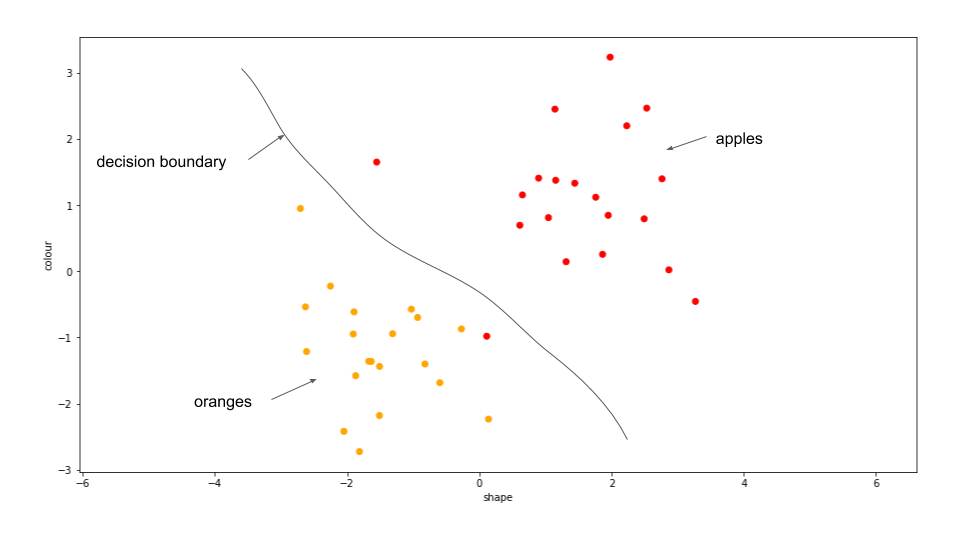
\includegraphics[width=0.8\textwidth]{oranges_and_apples_decision_boundary}
\end{figure}

Another class of data called non-IID data, where data samples are dependent and the sequence matters. These data are typically divided into training, validation and test sets for model training, where the type of data directly determines the best choice of model for mapping input to output. The choice of model also affects how the surface will look. A popular method of optimisation is gradient decent. Model updates are computed based on the first order parameter partial derivatives of the loss function.If the model only had three parameters, we could once again visualise how a possible loss surface might look. The job of the training algorithm, is to guide our model parameters toward a global minimum, in practice a local minimum is the best we can achieve.


%********************************** %Second Section  **************************************

\section{Deep Learning Models}

Deep learning models have become the preferred models for classification and regression tasks, and more broadly machine learning tasks. The reason for this is that deep models solve a major problem with shallow models - selecting the best features with which to represent samples ~\citep{Goodfellow-et-al-2016}. The problem of feature selection had resulted in a number of a methodology used during shallow model development: feature engineering. Feature engineering includes techniques such as bucketing, crossing, hashing and embedding ~\citep{murphy2012machine, Goodfellow-et-al-2016}. These techniques are designed to build sample representation that will result in high classification and regression accuracy. Deep models discovery optimal representations automatically, hence their superior performance on a number of machine learning tasks. \newline
Multilayer perceptrons (MLP) were the early deep learning models implemented as feed-forward neural networks consisting of $N$ layers, applied to an input vector $ x $. These models compute un-normalised scores known as logits, for each of the possible $ M $ outputs, classes and values in classification and regression respectively. They do this by executing a number of steps in an algorithm called the forward pass. Each step is called a layer, where an MLP can consist of a number of layers. A basic MLP consists of three of these layers, an input, hidden and output layer. The MLP computes a linear combinations of input features, then transforms the representation using a nonlinear hidden activation layer, before computing a linear combination of outputs. MLP models can be analytically defined as follows:

\begin{subequations}
\begin{gather}
	f_0=x \\
	f_i=\sigma_i(W_if_{i - 1} + b_i) \quad i \in [1, N]
\end{gather}
\end{subequations}

where $f_0$ is the input layers, $f_i$ is the respective computation layer. Each layer has a particular number,  $m_i$, of neurons. The parameters of a layer consist of a matrix $W_i \in \mathbb{R}^{m_i \times m_{i-1}}$ and bias vector $b_i \in  \mathbb{R}^{m_i}$. Each layer also has a non-linear activation function $\sigma_i$. \newline
Loss functions are used to train deep models under a supervised learning paradigm. The error computed by the loss is used in a process called back propagation - the computing of parametric first order partial derivatives, and the adjustment of the parameters in direction and magnitude of their respective derivative. Together the forward pass algorithm and back propagation, allow the automatic discovery of the most meaningful representation to compute the model output. We refer the reader to ~\citep{Goodfellow-et-al-2016} for a review on loss functions, as well as a more detailed discussion on the forward pass and back propagation. 

\subsection{Convolutional Networks}
The state-of-the-art in deep learning classification models is convolutional neural networks (CNN) \cite{reference}. CNNs are typically applied to object classification within images, and take advantage of the properties of object translation invariance and object location invariance \cite{reference}. These properties allow CNNs to perform robust classifications that generalise well across datasets. Translation invariance allows the CNN to build an object representation that is consistent under transformation, for example an image rotation would lead to a consistent final object representation being generated prior to logit computation for classification. Locality invariance allows the model to correctly identify an object no matter where it may reside with the boundaries of an image.\newline
These properties are possible because of how the final object representation is generated. CNNs perform a convolutional operation on an image, using a trainable image filter \cite{reference}. The operation generates feature map of the image that constructs latent object representations of the image. In practise these representations are chained together to produce more complex latent representations the deeper the CNN. \newline
% spatial and depth-wise convolutions
It is possible to decompose convolution operations into spatial and depth-wise convolutions \cite{reference}. A spatial convolution operates on different regions of an image, producing distinct representations for each region, for example and image can be divided into four regions, where a spatial convolution operates independently on each of these regions using region-specific filters.This operation produces four distinct feature maps which are later flattened into a single hidden layer representation, before begin run through a linear layer to generate the final logits. In a depth-wise convolution, the distinct convolutional feature maps are generated using the depth dimensions of the input image, typically three dimensions with images, the red, blue and green image channels in a colour image. Channel-specific filters are used to generate these feature maps and once again the future maps are flattened prior to computing logits for the model classes. \newline


%********************************** %Third Section  **************************************

\section{Regularisation}

%Deep Learning Best Practice}
 % initialisation e.g. xavier initialisation and truncated normal
 Xavier initilisation \cite{reference} is commonly used to initialise model parameters. This initialisation technique has the benefit of non-bias. It also influences the starting position on the loss surface increasing the likelihood of convergence. An other common parameter initialisation strategy is truncated normal initialisation \cite{reference}, where model paramaters are sampled from a univariate Gaussian distribution with mean zero and variance one. \newline
 % optimiser
The Adam \cite{reference} optimiser is commonly used for model training. This optimiser is an adaptive moment optimiser that scales the learning rate depending on the scale of parameter update changes. Other optimisers used for parameter updates include stochastic gradient descent \cite{reference}, ADAG-Grad \cite {reference} and RMS-Prop \cite{reference}. \newline
% learning rate scheduling
Learning rate scheduling \cite{reference}, the practice of reducing the learning rate after successive training cycles is now also common. It is implemented either as a continual process, where the learning rate is reduced by some proportion after every iteration, or on a step basis, where the learning rate is reduced by a proportion after every epoch. \newline
 % Hyperparameter optimistaion 
One of the most challenging aspects of model training is hyper parameter optimistaion \cite{reference}. Bayesian optimisation techniques have been used recently to overcome this problem \cite{reference}. Another hyper parameter search technique commonly used is random grid search \cite{reference}. This technique relies on iterations of hyper parameter sets that are uniformly sampled from range of available values. \newline

Model over parameterisation can lead to overfitting. This because the degrees of freedom available to estimate a function allow very complex nonlinear functions to be discovered, where these nonlinear functions or not representative of the generative process of the data at all \cite{reference}. These overfitting makes the model very sensitive to the training data, and results in poor generalisation across training, validation and testing data. This problem forms part of the broader bias/variance trade off, specifically high model variance due to over parameterisation. Deep learning models are particularly sensitive to overfitting given the high number of parameters present within the model. In order to compensate for this overfitting, it is common zero out a sample of neurons within a deep learning network. This has the effect of removing partial dependence between nodes deeper within the network, a form of principal component analysis generating independent latent features. These latent features result in a simpler model representation of the generative process of the data, and therefore allow it to generalise better across datasets. \newline

Batch normalisation attempts to account for internal covariance shift \cite{reference}. Batch normalisation is inspired from population based feature mean normalisation, when the entire population is taken into consideration when computing the mean and standard deviation of the values which the feature can take on within the dataset. When training a deep learning model, it is common to perform a uniform random shuffle of the training set, then subdivide that the set into mini-batches \cite{reference}. This is the same process of taking a uniform random sample batch from the training data. The size of the sample batch determines whether the normalised features remain within distributional alignment of the population. In order to compensate for the resultant loss computed after a foward pass, it is important to re-align feature vector parameters to the sample distribution mean and standard deviation estimators. The generated loss surface is thus a closer approximation to the true loss surface of the population, and subsequent parameter updates do not suffer from sample distributional distortion. This results in improved test accuracy as the model is able to more closely approximate the true distribution of the data. \newline 

\subsection{Loss Surface Analysis}
Defining an objective function is best informed by analysing the surface it generates. If the objective functions aims to minimise an error, it is a loss function, and if an objective function maximises an expected return, it is a reward function. Nonlinear factorisation models are commonly trained using loss functions presented in the following table:

\begin{table}[H]
	\centering
	\begin{tabular}{lllllllllll}
  		\textbf{Name} & \textbf{Expression} \\
  		\hline
  		Log (Nickel, Tresp, and Kriegel 2011) & $e^T_1W_r e_2$  \\
  		Constrastive Max Margin (Bordes et al. 2013) & $|| e_1 + w_r - e_2 ||$ \\
  		Cross Entropy (Socher et al. 2013) & $u^T_r f(e_1W_r^{[1..k]} e_2 + V_r \begin{bmatrix}e_1 \\ e_2\end{bmatrix} + b_r)$ \\
  		Binary Cross Entropy (Nickel, Rosasco, and Poggio 2016) & $r^T_p(e_s * e_o)$ \\
  		Softmax Cross Entropy (Balazevicl, Allen, and Hospedales 2018) & $f(vec(e_1 * vec^{-1}(w_rH))W)e_2$ \\
  		Sparse Categorical Cross Entropy (Magangane and Brink 2019) & $f(vec(e_1 * vec^{-1}(w_rH))W)f(vec(e_2 * vec^{-1}(w_rH))W)$
		\end{tabular}
 	\caption {Scoring functions of link prediction models. $*$ is the convolutional operator $F_r = vec^{-1}(w_rH)$ the matrix of relation specific convolutional filters, $f$ is a non-linear function}
\end{table} 

% loss function choice
The choice of loss function determines the training loss surface which in turn determines the expected model accuracy and convergence rate.

